Обозначим $a_k = E |\xi|^k$. 
Через $a_k$ выражаются все моменты. Например, $D\xi = E(\xi - E\xi)^2 = a_2 - a_1^2$.

Поэтому, верно следующее утверждение:
\begin{assertion}
Если $\exists E |\xi|^n < +\infty$, то конечны все моменты порядка не больше чем $n$.
\end{assertion}
\begin{proof}
$E |\xi|^n = \int\limits_{-\infty}^{+\infty} |x|^n \d F(x)$, он сходится. 
Если уменьшим $n$, то получим интеграл, который будет мажорироваться исходным везде, кроме отрезка $[-1; 1]$, значит интеграл на $\R \setminus [-1; 1]$ сходится.
Ну а на этом отрезке он конечен: $|x| \leq 1, \d F = p \d x$, интеграл плотности конечен, а мы его умножаем на что-то, не большее единицы.
\end{proof}

Как мы уже выяснили, просто матожидания недостаточно для того, чтобы однозначно определить случайную величину. 
Вопрос: а достаточно ли такого множества значений $\{a_k\}_{k=1}^\infty$?
В общем случае ответ -- нет, но:

\begin{theorem}
    Если $\varlimsup \frac{(E|\xi|^n)^\frac1n}{n} < +\infty$, то моменты определяют распределение.
\end{theorem}

\begin{theorem}[Неравенство Йенсена]

Пусть $g(x)$ выпукла вниз, тогда $g(E \xi) \leq E g(\xi)$
\end{theorem}
\begin{proof}
    Через каждую точку графика $g$ можно провести прямую, которая ограничивает график снизу (это будет просто касательная)
\begin{tikzpicture}
   \begin{axis}[
            xtick = \empty,    ytick = \empty,
           xlabel = {$x$},
           x label style = {at={(1,0)},anchor=west},
           ylabel = {$y$},
           y label style = {at={(0,1)},rotate=-90,anchor=south},
           axis lines=left,
           enlargelimits=0.2,
       ]
       \addplot[color=black,smooth,thick,-] {(x)^2};
       \addplot[mark=none, blue] coordinates {(6,20) (0,-4)};
        \addplot[blue, mark=*, only marks, nodes near coords = {$x_0$}, nodes near coords align={right}] coordinates {(2, 4)};
        %\draw[fill=blue] (6,20) circle (0.05); %node[right] {$x_0$};
    \end{axis}
\end{tikzpicture}    
    
    Возьмем точку $x_0 = E \xi$, через нее проходит прямая $ax + b$, ограничивающая график снизу: $ax + b \leq g(x), ax_0 + b = g(x_0)$.

    Тогда $$g(\xi) \geq g(E\xi) + a(\xi - E\xi)$$. 
    А теперь возьмем матожидание от обеих частей: 
    \begin{gather*}
    E(g(E\xi)) = g(E\xi) \text{как матожидание константы},\\
    E a(\xi - E\xi) = E a\xi - E aE\xi = E a\xi - E a\xi = 0
    \end{gather*}
    
    Откуда получаем $$g(E \xi) \leq E g(\xi)$$.
\end{proof}
\begin{conseq}[Неравенство Лягунова]
    $0 < s < t$. Тогда $$(E |\xi|^s)^\frac1s \leq (E |\xi|^t)^\frac1t$$.
\end{conseq}
\begin{proof}
    Применим Йенсена к $g(x) = |x|^\frac{t}{s}$
\end{proof}
\begin{conseq}
$|E\xi| \leq E|\xi|$.
\end{conseq}

\begin{theorem}[Неравенство Гёльдера]
    
$p > 1, q > 1, \frac1p + \frac1q = 1$, $E |\xi|^p, E|\eta|^q < \infty$. Тогда
$$E|\xi\eta| \leq (E |\xi|^p)^\frac1p (E |\eta|^q)^\frac1q$$
\end{theorem}
\begin{proof}
Если $\xi = 0$ или $\eta = 0$, то $0 \leq 0$. Иначе $E > 0$.

Заведем обозначения 
\begin{gather*}
\widetilde{\xi} = \frac{|\xi|}{(E |\xi|^p)^\frac1p}\\
\widetilde{\eta} = \frac{|\eta|}{(E |\eta|^q)^\frac1q}
\end{gather*}

Пусть $x, y, a, b > 0, a + b = 1$. Тогда верно $$x^ay^b \leq ax + by$$
Прологарифмируем это, получим $$a \ln x + b \ln y \leq \ln (ax + by)$$.

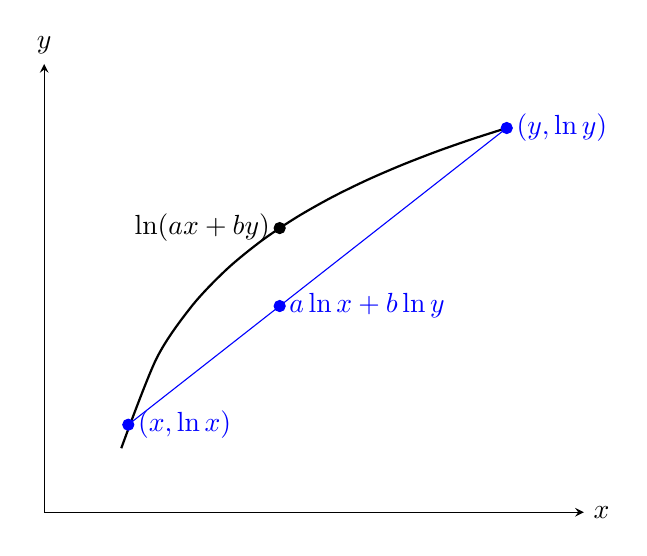
\begin{tikzpicture}
   \begin{axis}[
            xtick = \empty,    ytick = \empty,
           xlabel = {$x$},
           x label style = {at={(1,0)},anchor=west},
           ylabel = {$y$},
           y label style = {at={(0,1)},rotate=-90,anchor=south},
           axis lines=left,
           enlargelimits=0.2,
       ]
       \addplot[color=black,smooth,thick,-] {ln(x)};
       \addplot[mark=none, blue] coordinates {(0.5,-0.69314718056) (5,1.60943791243)};
        \addplot[blue, mark=*, only marks, nodes near coords = {$(x, \ln x)$}, nodes near coords align={right}] coordinates {(0.5,-0.69314718056)};
        \addplot[blue, mark=*, only marks, nodes near coords = {$(y, \ln y)$}, nodes near coords align={right}] coordinates {(5,1.60943791243)};
        \addplot[blue, mark=*, only marks, nodes near coords = {$a \ln x + b \ln y$}, nodes near coords align={right}] coordinates {(2.3,0.22788685663)};
        \addplot[black, mark=*, only marks, nodes near coords = {$\ln (ax+by)$}, nodes near coords align={left}] coordinates {(2.3,0.83290912293)};
   \end{axis}
\end{tikzpicture}

Вот эта картинка поясняет, почему неравенство действительно верно.
Возьмем
\begin{gather*}
a = \frac1p, b = \frac1q\\
x = \widetilde{\xi}^p, y = \widetilde{\eta}^q
\end{gather*}

Подставляем в неравенство, берем матожидание
\begin{gather*}
E ax = E \frac1p \frac{|\xi|^p}{E|\xi|^p} = \frac1p \frac{1}{E|\xi|^p} E |\xi|^p = \frac 1p\\
E \widetilde{\xi} \widetilde{\eta} \leq \frac1p \cdot 1 + \frac1q \cdot 1 = 1\\
E |\xi||\eta| \leq (E |\xi|^p)^\frac1p (E |\eta|^q)^\frac1q
\end{gather*}

\end{proof}

Другие характеристики распределения:
\begin{enumerate}
\item Носитель -- множество, куда мы попадаем с вероятностью 1.
\item Определим $z_p = \sup \{x \mid F_\xi (x) \leq p\}$. Тогда $z_\frac12$ -- медиана, $z_\frac14, z_\frac34$ -- квартили.
\item Мода = $\arg\max p_\xi(x)$.
\end{enumerate}


\begin{Def}
    $E{\vec{\xi}} = (E_{\xi_1}, \dots, E_{\xi_n})$.
\end{Def}
\begin{Def}
    Ковариацией пары случайных величин $\xi$ и $\eta$ называется $$cov(\xi, \eta) = E((\xi - E\xi)(\eta - E\eta) = E\xi\eta - E\xi E\eta$$ 
    В частости, при $\xi = \eta$ ковариация это дисперсия.
\end{Def}

\begin{theorem}[Свойства ковариации]
\begin{enumerate}
    \item $cov(\xi, \eta)$ -- билинейная по каждому аргументу, симметричная форма.
    \item Если $\xi, \eta$ независимы, то $cov(\xi, \eta) = 0$.
\end{enumerate}
\end{theorem}

\begin{Def}
    Рассмотрим случайный вектор $\xi = (\xi_1, \dots, \xi_n$, введем обозначение $\sigma_{ij} = cov(\xi_i, \xi_j)$

    $\sigma_{i,j=1}^n$ -- матрица ковариаций -- аналог дисперсии. Эта матрица симметрична и неотрицательно определена.
\end{Def}
Доказательство неотрицательной определенности:
\begin{proof}
Напоминание: $A$ неотрицательно определена, если $x^TAx \geq 0$ для любого вектора $x$. 

Возьмем случайную величину $\xi$ из векторного пространства, она представляется в виде линейной комбинации $\xi_i$. Тогда

$$0 \leq D(\sum\limits_{i = 1}^n c_i \xi_i) = E(\sum c_i (\xi_i - E \xi_i))^2 = \sum\limits_{i,j=1}^n c_i c_j \sigma_{ij}$$
Что и требовалось.
\end{proof}

\begin{Def}
    Коэффициентом корреляции называют $\rho(\xi, \eta) = \frac{cov(\xi, \eta)}{\sqrt{D_\xi D_\eta}}$
    
    Если $\rho(\xi, \eta) = 0$, то $\xi, \eta$ называют некоррелироваными.
\end{Def}
\begin{Rem}
    $|\rho| \leq 1$: применим неравенство Гёльдера с $p=q=2$ к $\xi - E\xi$ и $\eta - E\eta$.
\end{Rem}

\begin{Rem}
Из независимости следует некоррелируемость, а обратно нет.
Возьмем любое распределение $\xi$, симметричное относительно начала координат, $\rho(\xi, \xi) = 0$, так как \TODO на лекции так сказали, но это неверно, ниже правильный пример из гугла \TODO

Возьмем $\xi \sim U[-\pi, \pi]$, $\eta_1 = \sin \xi, \eta_2 = \cos \xi$. 
$\eta_1, \eta_2$ зависят, но корреляция равна нулю.
\end{Rem}                                                                                                                                         

\begin{Rem}

    $\rho$, по сути, является мерой линейной зависимости между случайных величин. 

    При этом, его модуль -- степень зависимости, а знак -- направление: если $\rho > 0$, то обе величины вместе растут/падают, иначе наоборот.
\end{Rem}

Рассмотрим задачу линейного прогноза: есть случайная величина $\eta$, мы ее не знаем, но хотим ее как-то угадать.
Для этого мы ее будем приближать какой-нибудь линейной функцией $g(\xi) = a\xi + b$. 

Надо взять и подобрать в каком-то смысле наилучшую функцию, то есть, оптимальные параметры $a$ и $b$. 
Будем минимизировать среднеквадратичное отклонение: $E(\eta - g(\xi))^2$
\begin{Rem}
А еще это иногда называют задачей линейной регрессии, например, встречается в машинном обучении.
\end{Rem}

Упражнение: если $E(\eta - a^*\xi -b^*)^2$ -- минимум ($a^*, b^*$) -- оптимальные параметры), то $a^* = \frac{cov(\xi, \eta)}{D\xi}, b^* = E\eta - a^*E\xi$.

Можно заметить, что $E(\eta - a^*\xi -b^*)^2 = (1 - \rho^2) D\eta$ (просто раскроем скобки). Тогда $\eta =  a\xi + b$ тогда и только тогда когда $|\rho| = 1$

\begin{Rem}
Наличие корелляции вовсе не гарантирует какую-либо причинно-следственную связь. 

Например, есть известная шутка про то, что численность пиратов уменьшается из-за глобального потепления (корелляция то действительно есть между этими двумя величинами, а вот связь -- вряд ли) 
\end{Rem}

\begin{Def}
Пространство $L^2$ случайных величин -- пространство величин с конечным вторым моментом: $E \xi^2 < \infty$
\end{Def}

Упражнение: в нем $cov(\xi, \eta)$ -- скалярное произведение (можно просто руками проверить все свойства скалярного произведения).

``Длина'' $\xi$ это $\sqrt{(\xi, \xi)} = \sqrt{D\xi} = \sigma \xi$ -- среднеквадратичное отклонение.

``Косинус угла'' это $\rho(\xi, \eta)$, некореллируемые величины -- перпендикулярные.

Лучшее линейное приближение $\eta$ -- проекция на плоскость $a\xi + b = 0$: расстояние будет минимальным, когда получится перпендикуляр.
А он вылезает как разность вектора и проекции.  \TODO картинку бы \TODO


\section{Общий (функциональный) прогноз}

Более общая задача: теперь $g(\xi)$ -- произвольная борелевская фукнция, не обязательно линейная.
И хотим приблизить $\eta$ этой функцией.    

Оказывается, что решением этой задачи является условное матожидание.

\begin{Def}
Пусть $\forall x\colon g(x) = E(\eta \mid \xi = x)$. Тогда $E(\eta \mid \xi) = g(\xi)$. Это и называется условным матожиданием.
\end{Def}

\begin{Def}
    Пусть $\mathbb{A} \subset \mathbb{F}$ -- $\sigma$-алгебра.

    $\eta_\mathbb{A} = E(\eta \mid \mathbb{A})$ -- $\mathbb{A}$-измеримая случайная величина (то есть $\forall B \in \mathbb{B}\colon E(\eta \mid \mathbb{A})^{-1}(B) \in \mathbb{A}$),
    такая что $\forall A \in \mathbb{A}\colon E\eta \mathbb{1}_A = E\eta_\mathbb{A} \mathbb{1}_A$
\end{Def}
\begin{exmp}
    Пусть $\Omega = \R$
    \begin{enumerate}
    \item
        $\mathbb{A} = \{\varnothing, \R\}$, тогда $\eta_\mathbb{A} = E\eta$
    \item
        $\mathbb{A} = \sigma(\{[k, k + 1)\})$. Новая случайная величина должна быть постоянна на этих интервалах (потому что она $\mathbb{A}$-измерима), 
        и при этом интегралы должны совпадать с интегралами исходной величины, откуда получаем значение на каждом интервале.
    \item   
        $\mathbb{A} = \{A \colon A = -A\}$, $\eta_\mathbb{A}(w) = \frac{\eta(w) + \eta(-w)}{2}$
    \end{enumerate}
\end{exmp}

\begin{Def}
    $\Xi$ -- набор множеств, тогда $E(\eta \mid \Xi) = E(\eta \mid \sigma(\Xi))$

    $\xi$ -- случайная величина, тогда $E(\eta \mid \xi) = E(\eta \mid \mathbb{F}_\xi)$
\end{Def}
\begin{Rem}
    Это определение и первое равносильны, доказывать это мы, конечно же, не будем.
\end{Rem}